\section{Attacco all'autenticazione delle reti 2G-4G}
Le reti cellulari dal 2G al 4G condividono lo stesso schema architetturale generale, per questo gran parte delle vulnerabilità che vengono
utilizzate negli attacchi \textit{Denial of Service} sono comuni.
Ci sono numerosi modi per fare un attacco di tipo \textit{Denial of Service} alle reti cellulari, gran parte di questi utilizzano
una \textit{botnet} per esasperare di richieste i componenti critici del \textit{network}, creando così i \textit{Distributed Denial of Service}.\\


\subsection{IMSI stealing}
\cite{dos-imsi}
\cite{imsi-catcher}

\subsection{Botnet}
\cite{measuring-dos}

\subsection{Attacco alle reti con dispositivi SIM-less}
\cite{gsm-dos-simless}
In \cite{umts-dos} è descritto un attacco di tipo \textit{Denial of Service} alle reti UMTS, in particolare al
sistema di identificazione degli utenti. \\
Lo studio dmostra che è possibile generare delle onerose computazioni all'interno dell'infrastruttura cellulare senza 
disporre di dispositivi con delle SIM valide. Inoltre, nell'attacco trattato i dispositivi che sono necessari per avere una 
degradazione del servizio sono un numero nettamente minore rispetto allo stato dell'arte, ciò rende la sua realizzazione molto
più accessibile. Con l'inserimento di SIM valide nei dispositivi è possibile ridurre il numero di interfacce UMTS necessarie per compiere 
l'attacco con successo, infatti queste si riducono a qualche centinaio.
Visto il numero contentuto di dispositivi che sono necessari per effettuare l'attacco, si può evitare di usare una \textit{botnet} rendendo l'attacco
molto più stabile e quindi più pericoloso.\\
L'attacco ha come obbiettivo la degradazione di uno dei componenti centrali dell'architettura UMTS: la HLR. Questo componente è il più semplice da 
attaccare poichè avvengono continue interrogazioni durante tutta la fase di autenticazione e identificazione del MS.
Siccome non si tratta di una \textit{botnet} è stata fondamentale l'analisi della capacità dei canali di comunicazione in modo tale da scoprire eventuali
\textit{bottleneck} che minerebbero l'esecuzione dell'attacco.
\begin{figure}[h]
    \centering
    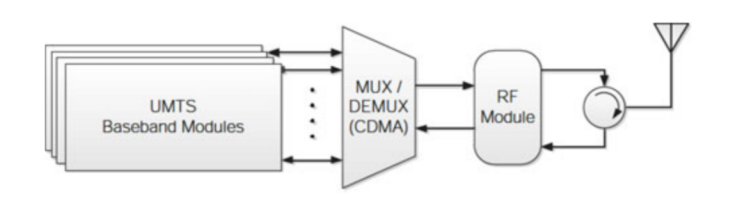
\includegraphics[width=0.5\textwidth]{images/umts-dos-device.png}
    \caption{Dispositivo per l'attacco DOS alle reti UMTS\cite{umts-dos}}
\end{figure}\\
I risultati ottenuti si basano su stime dei tempi di risposta dei componenti architetturali trattati. Questo perchè i vari MNOs non forniscono nessuna 
informazione ufficiale riguardo le \textit{performance}.